\documentclass[11pt,compress,t,notes=noshow, aspectratio=169, xcolor=table]{beamer}

\usepackage{../../style/lmu-lecture}
% Defines macros and environments
% This file is included in slides and exercises

% Rarely used fontstyle for R packages, used only in 
% - forests/slides-forests-benchmark.tex
% - exercises/single-exercises/methods_l_1.Rnw
% - slides/cart/attic/slides_extra_trees.Rnw
\newcommand{\pkg}[1]{{\fontseries{b}\selectfont #1}}

% Spacing helpers, used often (mostly in exercises for \dlz)
\newcommand{\lz}{\vspace{0.5cm}} % vertical space (used often in slides)
\newcommand{\dlz}{\vspace{1cm}}  % double vertical space (used often in exercises, never in slides)
\newcommand{\oneliner}[1] % Oneliner for important statements, used e.g. in iml, algods
{\begin{block}{}\begin{center}\begin{Large}#1\end{Large}\end{center}\end{block}}

% Don't know if this is used or needed, remove?
% textcolor that works in mathmode
% https://tex.stackexchange.com/a/261480
% Used e.g. in forests/slides-forests-bagging.tex
% [...] \textcolor{blue}{\tfrac{1}{M}\sum^M_{m} [...]
% \makeatletter
% \renewcommand*{\@textcolor}[3]{%
%   \protect\leavevmode
%   \begingroup
%     \color#1{#2}#3%
%   \endgroup
% }
% \makeatother


\title{Interpretable Machine Learning}
% \author{LMU}
%\institute{\href{https://compstat-lmu.github.io/lecture_iml/}{compstat-lmu.github.io/lecture\_iml}}
\date{}

\def\firstrowcolor{}
\def\secondrowcolor{}
\def\thirdrowcolor{}
\def\fourthrowcolor{}

\definecolor{winter}{RGB} {243,117,108}
\definecolor{spring}{RGB} {121,174,65}
\definecolor{summer}{RGB} {25,188,195}
\definecolor{fall}{RGB} {166,128,185}
\setlength{\leftmargini}{1.5em}
\setlength{\leftmarginii}{1em}
\begin{document}

\newcommand{\titlefigure}{figure/lm_example}
\newcommand{\learninggoals}{
\item LM basics and assumptions
\item Interpretation of main effects in LM
\item What are significant features?
}

\lecturechapter{Linear Regression Model}
\lecture{Interpretable Machine Learning}




\begin{frame}[c]{Linear Regression}
% https://towardsdatascience.com/assumptions-of-linear-regression-fdb71ebeaa8b
% https://www.statology.org/linear-regression-assumptions/
% https://link.springer.com/book/10.1007/978-3-642-34333-9
%\textbf{Model formula}
    %$$\mathbb{E}_Y(Y \vert X) = \theta_0 + \theta_1 x_1 + \theta_2 x_2 + \ldots + \theta_p x_p + \epsilon = X^T\mathbf{\theta} + \epsilon$$

\begin{columns}[T, totalwidth = \linewidth]
\begin{column}{0.58\linewidth}
$$y = \theta_0 + \theta_1 x_1 + \theta_2 x_2 + \dots + \theta_p x_p + \epsilon = \xv^\top \boldsymbol{\theta} + \epsilon$$

 \begin{itemize}
        %\item $\mathbb{E}_Y(Y \vert X)$ expected value of target given features $X$
        \item $y$: target / output
        \item $\epsilon$: remaining error / residual %(e.g., due to noise)
        \item $\theta_j$: weight of input feature $x_j$ (intercept $\theta_0$)\\
        $\leadsto$ model consists of $p+1$ weights
        %\item Model equation is additive and identical across entire input space
        %\pause
        % \item Polynomial regression extends equation above by
        % \begin{itemize}
        % \item \textbf{higher order main effects} which have their own weights (e.g., quadratic: $\theta_{x_j^2} \cdot x_j^2$)
        % \item \textbf{interaction effects} (e.g., 2-way interaction: $\theta_{x_i, x_j} \cdot x_i \cdot x_j$)
        % \end{itemize}
    \end{itemize}
\end{column}
\begin{column}{0.42\linewidth}
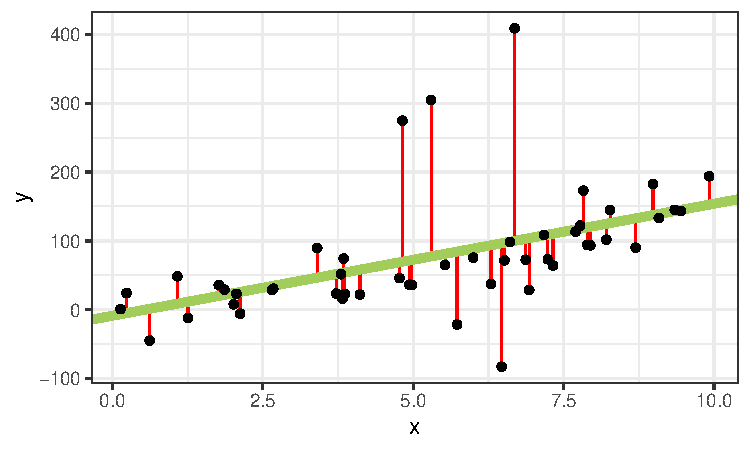
\includegraphics[width=\linewidth]{figure/lm_example.pdf}
\end{column}
\end{columns}
   
   \vspace*{0.2cm} 
   \pause
    \textbf{Properties and assumptions} \citebutton{Faraway (2002), Ch. 7}{https://cran.r-project.org/doc/contrib/Faraway-PRA.pdf} \citebutton{Checking assumptions in R \& Python}{https://towardsdatascience.com/assumptions-of-linear-regression-fdb71ebeaa8b}
    \begin{itemize}[<+->]
    \item \textbf{Linear} relationship between features and target
    %Predictions are \textbf{linear} combination of features $\leadsto$ 
    %Model equation is additive and linear w.r.t. features% and identical across entire input space
    \item $\epsilon$ and $y \vert \xv$ are \textbf{normally} distributed with \textbf{constant variance} (homoscedastic)\\
    $\leadsto$ $\epsilon \sim N(0, \sigma^2) \; \Rightarrow \; (y \vert \xv) \sim N(\xv^\top \theta, \sigma^2)$\\
    $\leadsto$ if violated, inference-based metrics (e.g., p-values) are invalid
    %\item Error terms are assumed to have a \textbf{constant variance} over the entire feature space %(homoscedasticity)
    \item Independence of observations (e.g., no repeated measurements) %(e.g., no autocorrelated error terms)
    \item Features $x_j$ independent from error term $\epsilon$
    \item No or little multicollinearity (i.e., no strong feature correlations)
    % free of measurement error assumption: https://indigo.uic.edu/articles/thesis/Measurement_Error_in_Generalized_Linear_Models/17025971/1/files/31488719.pdf
    % \item Note: For inference-based metrics (t-statistic, p-values, confidence intervals) to be valid, the error term needs to be normally distributed, i.e., $\epsilon \sim N(0, \sigma^2) \; \Rightarrow \; (y \vert x) \sim N(x^T \theta, \sigma^2)$\\
%$\leadsto$ Restricts use of LMs in practice as distribution of error is a prior assumption about data
        % \item Properties and assumptions:
        % \begin{itemize}
        %     \item linear
        %     \item normality assumption of the target % not true...
        %     \item homoscedastic (i.e., constant variance)
        %     \item independence of features
        %     \item fixed features (i.e., free of noise)
        %     \item no strong correlation of features
        % \end{itemize} 
    \end{itemize}

\end{frame}

%------------------------------------------------------------------
%------------------------------------------------------------------

\begin{frame}{Linear Regression - Interpretation}

$$y = \theta_0 + \theta_1 x_1 + \theta_2 x_2 + \dots + \theta_p x_p + \epsilon = \xv^\top \thetab + \epsilon$$

    Interpretation of weights (\textbf{feature effects}) depend on type of feature:
    \begin{itemize}[<+->]
        \item \textbf{Numerical $x_j$}: Increasing $x_j$ by one unit changes outcome by $\theta_j$, ceteris paribus \\ (\textit{ceteris paribus} (c.p.) means "everything else held constant".)
        \item \textbf{Binary $x_j$}: Weight $\theta_j$ is active or not (multiplication with 1 or 0)\\
        $\leadsto$ reference category $x_j = 0$
    \end{itemize}
%
\begin{columns}[T, totalwidth = \textwidth]
\begin{column}{0.62\textwidth}
    \begin{itemize}
        \item<3-> %Categorical: One-hot-encoding of $L-1$ new features for $L$ categories (dummy encoding) \\
        \textbf{Categorical feature $x_j$ with $L$ categories}: 
        \begin{itemize}
            \item Create $L-1$ one-hot-encoded features $x_{j,1}, \hdots, x_{j,L-1}$ (each having its own weight)
            \item Left out cat. is reference ($\hat =$ dummy encoding)
            \item[$\leadsto$] Interpretation:
        Outcome changes by $\theta_{j,i}$ for category $i$ compared to reference cat.,  c.p.
        \end{itemize}
        %$x_{j,l}, \forall l \in \{1, \hdots, L-1\}$ (with weight $\theta_{j,l}$), left out category is reference ($\hat =$ dummy encoding)       
        % (for any of the $L-1$ categories):
        %Predicted outcome changes for $l$-th category compared to the reference category by its weight $\theta_{j,l}$ c.p.
        %Predicted outcome changes for category $x_{j,l}$ compared to the reference category by $\theta_j$ c.p.
        \item<4> \textbf{Intercept $\theta_0$}: Expected outcome if all feature values are set to 0 %(baseline) %reflects expected features values if features were standardised (0-mean, 1-stdev)
        %\item Note: In case of higher order or interaction effects, weights cannot be interpreted in isolation
    \end{itemize}
\end{column}
\begin{column}{0.38\textwidth}
%\begin{center}
        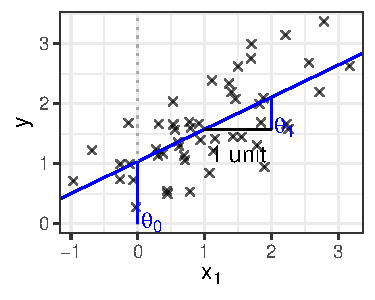
\includegraphics[trim={0 5 0 5},clip, width = \textwidth]{figure/reg_lm_plot_interpreted.pdf}\\
        % Bild aus I2ML: supervised-regression
        %figure/plot_lin_effect.pdf} \\
        %Boxplot of $\hat\theta_j x_j$-values (scale invariant)
        %$\leadsto$ Comparable feature contributions w.r.t. $\hat y$
    %\end{center}
\end{column}
\end{columns}
    
\end{frame}

     
\begin{frame}{Linear Regression - Interpretation}
\vspace{-0.2cm}
$$y = \theta_0 + \theta_1 x_1 + \theta_2 x_2 + \dots + \theta_p x_p + \epsilon = \xv^\top \thetab + \epsilon$$
    \textbf{Feature importance}:
    \begin{columns}[T, totalwidth=\textwidth]
    \begin{column}{0.6\textwidth}
    \begin{itemize}
        \item Absolute \textbf{t-statistic} value: $\hat\theta_j$ scaled with standard error ($SE(\hat\theta_j)$ $\hat =$ reliability of estimate) 
    $$|t_{\hat\theta_j}| = \left| \frac{\hat\theta_j}{SE(\hat\theta_j)} \right|$$
        \item High $t$-values $\Rightarrow$ important (significant) feat.
    \end{itemize}
    \end{column}
    \begin{column}{0.4\textwidth}
    %\vspace{-0.2cm}
    %\begin{center}
        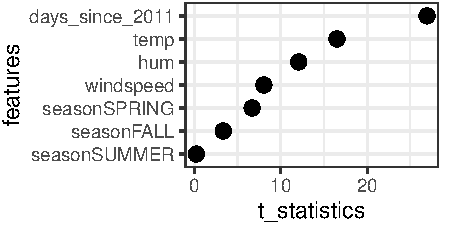
\includegraphics[width=\textwidth]{figure/t_stat.pdf} 
    %\end{center}
    \end{column}
    \end{columns}
    \vspace{0.3cm}
    \only<2->{
    \begin{columns}[T, totalwidth=\textwidth]
    \begin{column}{0.6\textwidth}
    \begin{itemize}
        \item \textbf{p-value}: 
        probability of obtaining a more extreme test statistic assuming $H_0$ is correct (here: $\theta_j =0$, i.e., feat. $j$ not significant)
        %probability of obtaining a test statistic that is more extreme (values that speak against $H_0$) as the test statistic computed from the sample, assuming $H_0$ (here: $\theta_j =0)$ is correct.
        \\
        $\leadsto$ High $|t|$ $\Rightarrow$ small p-val. (speak against $H_0$)
        %\item The smaller the p-value, the less likely it is to obtain a more extreme test statistic
    \end{itemize}
    \end{column}
    \begin{column}{0.4\textwidth}
    %\vspace{-0.3cm}
    %\begin{center}
        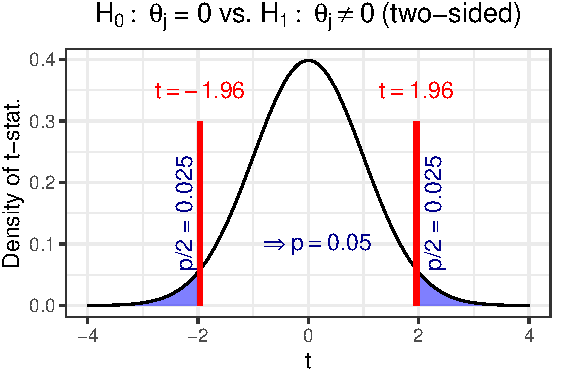
\includegraphics[width=\textwidth]{figure/p-value.pdf}
    %\end{center}
    \end{column}
    \end{columns}}
\end{frame}


\begin{frame}{Example: Linear Regression - Main Effects}

\textbf{Bike data}: predict no. of rented bikes using 4 numeric, 1 categorical feat. (season)

\medskip 

% \begin{footnotesize}
% $$
% \hat y = \hat \theta_0 + \hat \theta_1 \mathds{1}_{(seas = SPRING)} + \hat \theta_2 \mathds{1}_{(seas = SUMMER)} + \hat \theta_3 \mathds{1}_{(seas = FALL)} + \hat \theta_4 temp + \hat \theta_5 hum + \hat \theta_6 windspeed + \hat \theta_7 days\_since\_2011
% $$
% \end{footnotesize}
\begin{columns}[T, totalwidth=\textwidth]
\begin{column}{0.43\linewidth}
\vspace*{-0.3cm}
\begin{align*}
\hat y = 
& \hat \theta_0 + 
\hat \theta_1 \mathds{1}_{x_{season} = SPRING} +\\
& 
\hat \theta_2 \mathds{1}_{x_{season} = SUMMER} +\\
& 
\hat \theta_3 \mathds{1}_{x_{season} = FALL} + 
\hat \theta_4 x_{temp} + \\
& 
\hat \theta_5 x_{hum} + 
\hat \theta_6 x_{windspeed} + \\
& 
\hat \theta_7 x_{days\_since\_2011}
\end{align*}
\end{column}
\begin{column}{0.57\linewidth}
  \centering
\begin{scriptsize}
%\begin{overlayarea}{\textwidth}{\textheight}
%\begin{table}[ht]
\only<2>{\def\firstrowcolor{\rowcolor{lightgray}}}
\only<3>{\def\secondrowcolor{\rowcolor{lightgray}}}
\only<4>{\def\thirdrowcolor{\rowcolor{lightgray}}}
\begin{tabular}{rrrrr}
  \hline
 & Weights & SE & t-stat. & p-val. \\
 \hline
\firstrowcolor (Intercept) & 3229.3 & 220.6 & 14.6 & 0.00 \\ 
\secondrowcolor seasonSPRING & 862.0 & 129.0 & 6.7 & 0.00 \\ 
  seasonSUMMER & 41.6 & 170.2 & 0.2 & 0.81 \\ 
  seasonFALL & 390.1 & 116.6 & 3.3 & 0.00 \\ 
\thirdrowcolor temp & 120.5 & 7.3 & 16.5 & 0.00 \\ 
  hum & -31.1 & 2.6 & -12.1 & 0.00 \\ 
  windspeed & -56.9 & 7.1 & -8.0 & 0.00 \\ 
  days\_since\_2011 & 4.9 & 0.2 & 26.9 & 0.00 \\
   \hline
\end{tabular}
%\end{table}
%\end{overlayarea}
\end{scriptsize}
\end{column}
\end{columns}
%\vspace*{-0.3cm}
\pause

\lz
%\begin{columns}[T, totalwidth=\textwidth]
%\begin{column}<5>{0.46\textwidth}
%\textbf{Vis.}: Boxplot of $\hat\theta_j x_j$-values (scale invariant)\\
%weights multiplied by actual feature value (better comparable due to different scales)
%$\leadsto$ Comparable feature contributions w.r.t. $\hat y$

%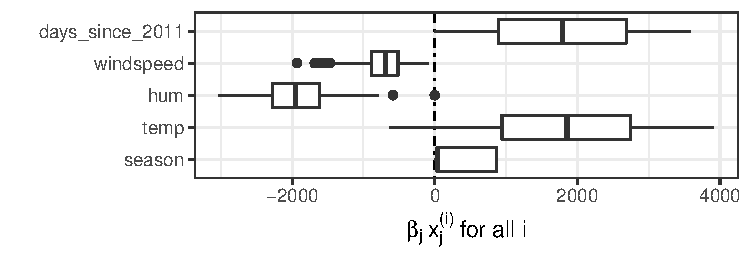
\includegraphics[width = \textwidth]{figure/plot_lin_effect.pdf}
%   \begin{center}
%   % Effect of $i$-th observation $= \theta_j x_j^{(i)}$\\

%     %$\leadsto$ Better comparability due to different scales
%   \end{center}
%\pause
%\verbatiminput{figure/lm_output.txt}
%\end{column}\hfill
%\begin{column}{0.54\textwidth}  %%<--- here
\textbf{Interpretation:}

\begin{itemize}[<+->]
    \item \textbf{Intercept}:
    If all feature values are 0 (and season is \code{WINTER} $\hat =$ reference cat.), the expected number of bike rentals is $\hat\theta_0 = 3229.3$
    \item \textbf{Categorical}: Rentals in \code{SPRING} are by $\hat\theta_1 = 862$ higher than in \code{WINTER}, c.p.
    \item \textbf{Numerical}: Rentals increase by $\hat\theta_4 = 120.5$ if \code{temp} increases by 1 $^{\circ}$C, c.p.
    %If the temperature increases by 1 order Celsius, the number of bike rentals increases by 120.5 c.p.

\end{itemize}
%\end{column}
%\end{columns}
\end{frame}

\endlecture
\end{document}
